\newpage
\section{神经网络基础类型}

\subsection{多层感知机 (MLP)}
输入: vector $v\in R^{1\times C}$
\begin{align*}
    \begin{array}{ll}
        o_1=ReLU(v\cdot W_1) & W_1 \in \mathbb{R}^{C\times C'}\\
        o_2=ReLU(o_1\cdot W_1) & W_2 \in \mathbb{R}^{C'\times C''}\\
        o_3=ReLU(o_2\cdot W_1) & W_3 \in \mathbb{R}^{C''\times C'''}
    \end{array}
\end{align*}

\begin{figure}[!htb]
    \centering
    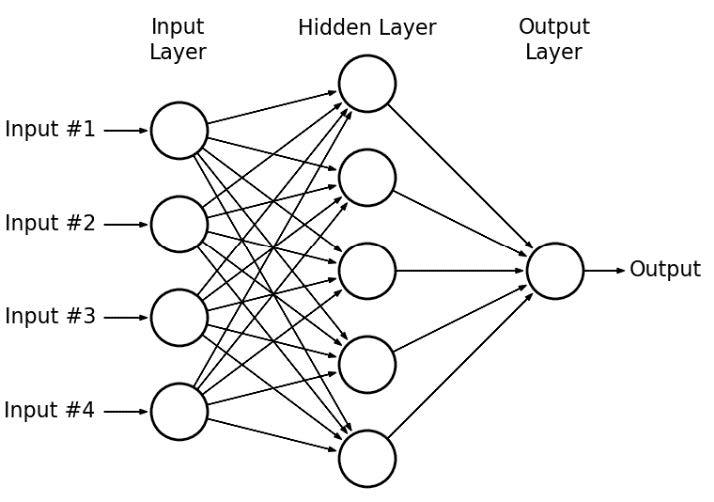
\includegraphics[width=0.309\textwidth]{pic/DL2/MLP.jpg}
    \caption{MLP}
\end{figure}


非线性函数 e.g.
\begin{enumerate}
    \item sigmoid
    \item tanh
    \item ReLU
    \item LeakyReLU
\end{enumerate}

学习的根本是收集收益大的 activation, 将重要的信号汇聚到一起. 前两者限制了重要信号的大小, 产生了损失. 

\subsection{卷积神经网络 (CNN)}
三维的叫 tensor $\mathbf{I}$, 二维的叫矩阵 $W$, 一维的叫向量 $\mathbf{v}$?


以当前像素为中心, 在大小为$[h,w]$的局部区域内, 每个方向和距离$(i, j)$安排一参数$W^{(i,j)}$
\begin{align*}
    \mathbf{I}'^{(x,y)}=\sum_{i=-\lfloor h/2\rfloor}^{\lfloor h/2\rfloor}\sum_{j=-\lfloor w/2\rfloor}^{\lfloor w/2\rfloor}W^{(i,j)}\cdot \mathbf{I}^{(x+i, y+j)}+b^{(i,j)}
\end{align*}
$\mathbf{I}\in \mathbb{R}^{C\times H\times W}$, $\mathbf{I}^{(x,y)}\in R^{C}$, $W \in \mathbb{R}^{h\times w\times C' \times C}$, $W^{i,j}\in \mathbb{R}^{C'\times C}$. 

CNN可以感受到方向和距离. 

\begin{enumerate}
    \item Padding (填充), 一般用0填充. 
    \item Stride: 走的距离, 控制下采样的大小
    \item Dilation (膨胀): 更大的卷积核, 更大的感受野, 但参数增多少. 
    \item Pooling (池化): Max or Average, 可以用卷积取代
\end{enumerate} 

e.g. AlexNet

\subsection{循环神经网络 (RNN)}
\begin{align*}
    h_t&=\tanh (W_1 \cdot x_t + W_2 \cdot h_{t-1} +b)\\
    o_t&=h_t
\end{align*}
\begin{figure}[!htb]
    \centering
    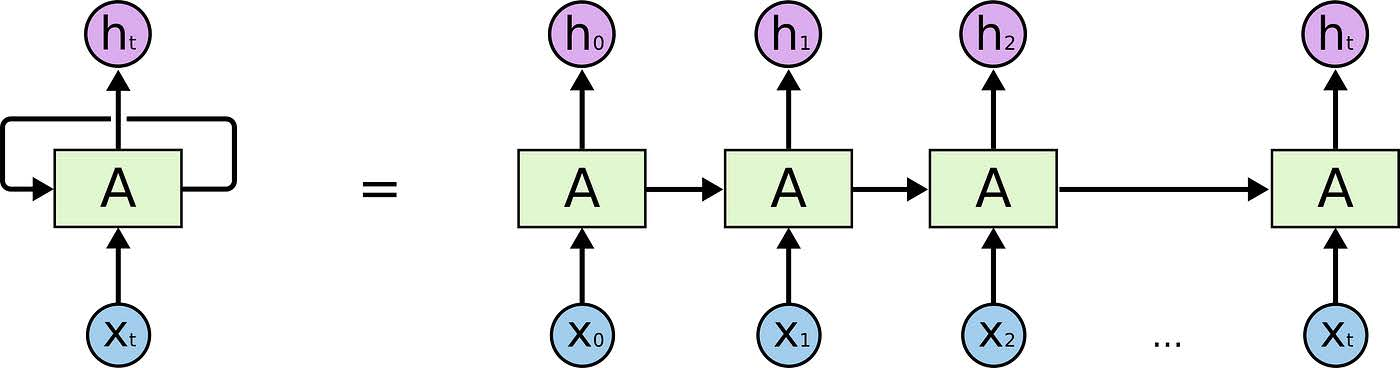
\includegraphics[width=0.42\textwidth]{pic/DL2/RNN}
    \caption{RNN}
\end{figure}

变体: LSTM, GRU

\subsubsection{长短记忆网络 (LSTM)}
\begin{figure}[!htb]
    \centering
    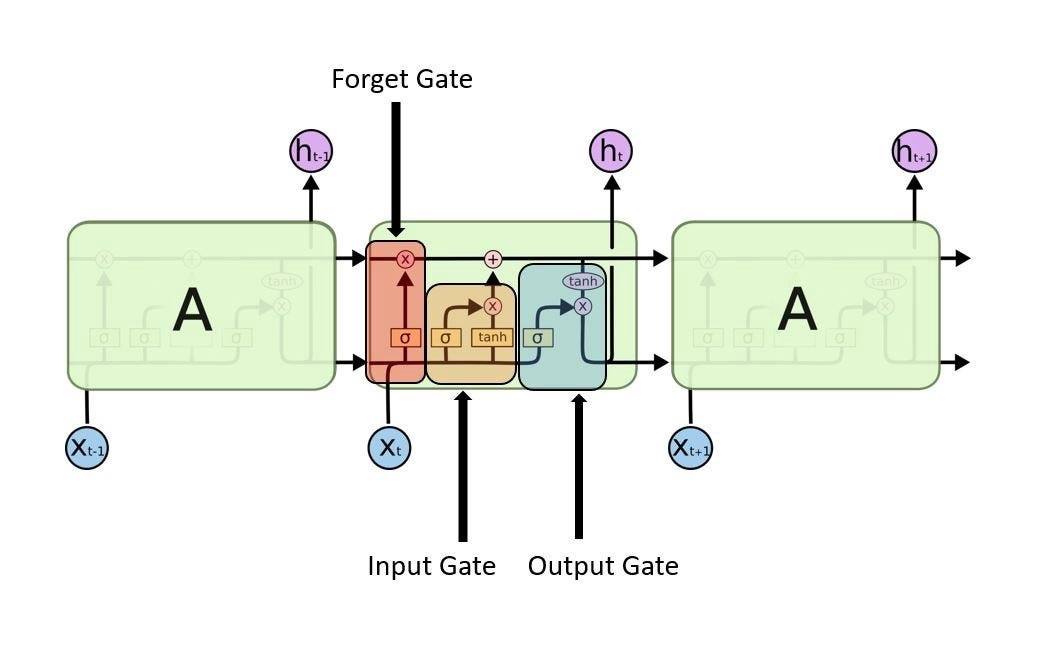
\includegraphics[width=0.309\textwidth]{pic/DL2/LSTM}
    \caption{LSTM}
\end{figure}


\subsubsection{Gated Recurrent Unit (GRU)}
\begin{figure}[!htb]
    \centering
    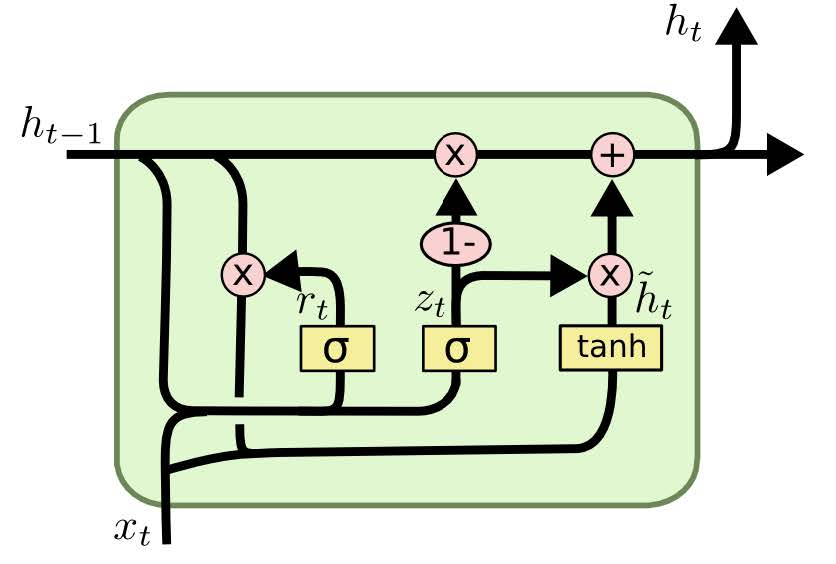
\includegraphics[width=0.309\textwidth]{pic/DL2/GRU}
    \caption{GRU}
\end{figure}



\subsection{图神经网络 (GNN)}
\begin{figure}[!htb]
    \centering
    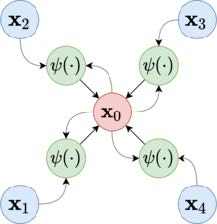
\includegraphics[width=0.309\textwidth]{pic/DL2/GNN}
    \caption{GNN}
\end{figure}


\begin{align*}
    h_u=\phi\left( x_u, \bigoplus_{v\in N_u}\psi(x_u, x_v, e_{uv}) \right)
\end{align*}
$x_u$为中心点, $x_v$为邻居点, $e_{uv}$为边的信息, 是vector. 

\subsection{Transformer}
自注意力(自适应计算感受野)
{\small
\begin{align*}
    \begin{array}{rl}
        \text{Image: }& I \in \mathbb{R}^{C\times N}\ (N=H\times W)\\
        \text{绝对位置编码: }& I^{(x,y)}=I^{(x,y)}+Emb(x,y)\\ 
        \text{Query: }& Q=W_q\cdot I \in \mathbb{R}^{C'\times N},\ W_q\in \mathbb{R}^{C'\times C}\\
        \text{Key: }& K=W_k\cdot I \in \mathbb{R}^{C'\times N},\ W_k\in \mathbb{R}^{C'\times C}\\
        \text{Scaled Dot Product: }& P=\frac{Q^T\cdot K}{\sqrt{C'}}\in \mathbb{R}^{N\times N}\\
        \text{Attention: }& A=softmax(P)\in \mathbb{R}^{N\times N}\\
        \text{Value: }& V=W_v\cdot I \in \mathbb{R}^{C' \times N},\ W_v\in \mathbb{R}^{C'\times C}\\
    \end{array}
\end{align*}
}Value 没有对方向, 距离信息的编码
\begin{align*}
    F_a=\sum_{b=1}^N A_{ab}\times V_b
\end{align*}
$V_b$是 patch $b$的表征, $A_{ab}$ 是patch $a$与patch $b$直接的相关性. 最终求和得以patch $a$为中心的相关区域表征. 

\begin{figure}[!htb]
    \centering
    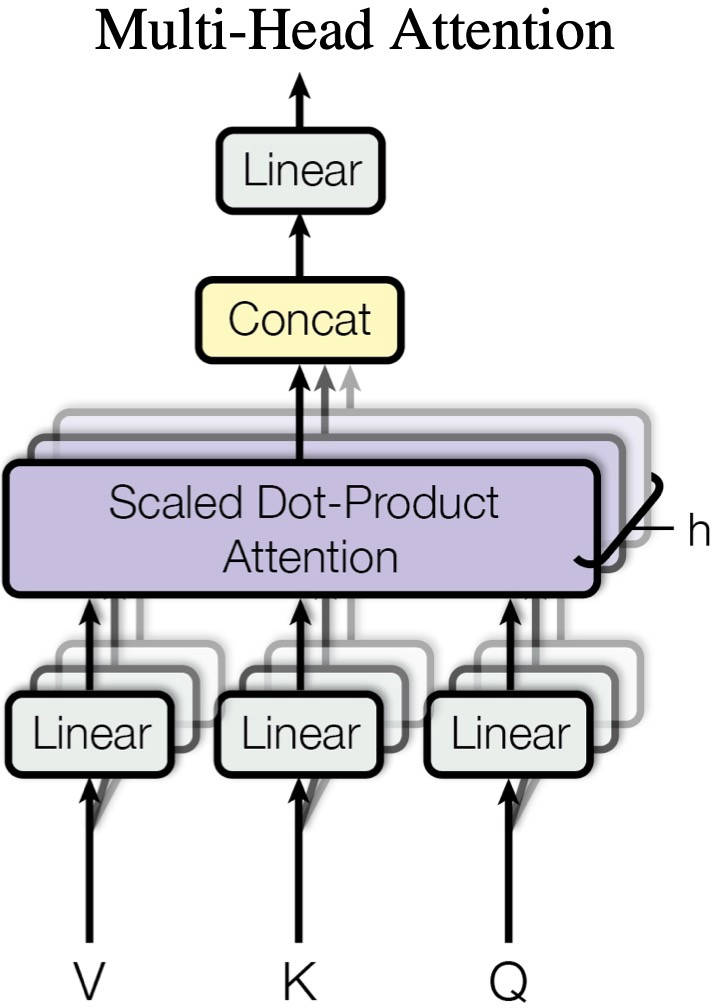
\includegraphics[width=0.309\textwidth]{pic/DL2/Multi-Head Attention}
    \caption{Multi-Head Attention}
\end{figure}


\subsection{总结}

\subsubsection{卷积与 Transformer 的 统一}
\begin{align*}
    I_a=\sum_{b=1}^N A_{ab}\times W^{(b-a)}\times I_b
\end{align*}


\subsubsection{相对位置与绝对位置}
绝对位置有效是因为数据足够多, 可以提供清晰的拟合对象

\subsubsection{Transformer模板}

\begin{figure}[!htb]
    \centering
    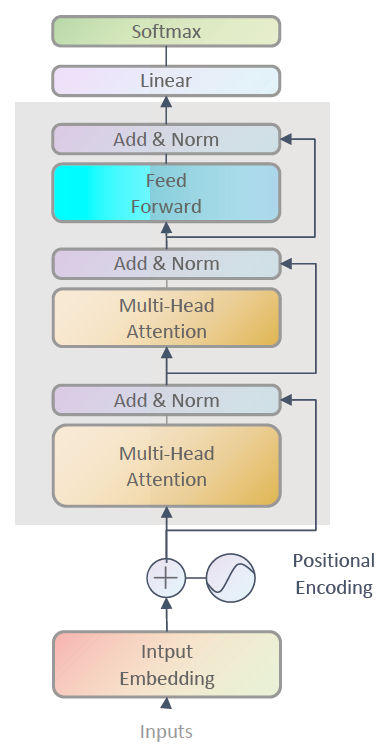
\includegraphics[width=0.24\textwidth]{pic/DL2/Transformer}
    \caption{Transformer}
\end{figure}
